\chapter{Introduction}
\par In Physiotherapy, tracking Range of Motion (ROM) is a standard approach to measuring progress in patient therapy. Often, ROM is measured subjectively and documentation is inconsistent between clinicians. Physios might come to wrong conclusions if ROM is tracked incorrectly between therapy sessions.

\begin{figure}[htbp]
	\centerline{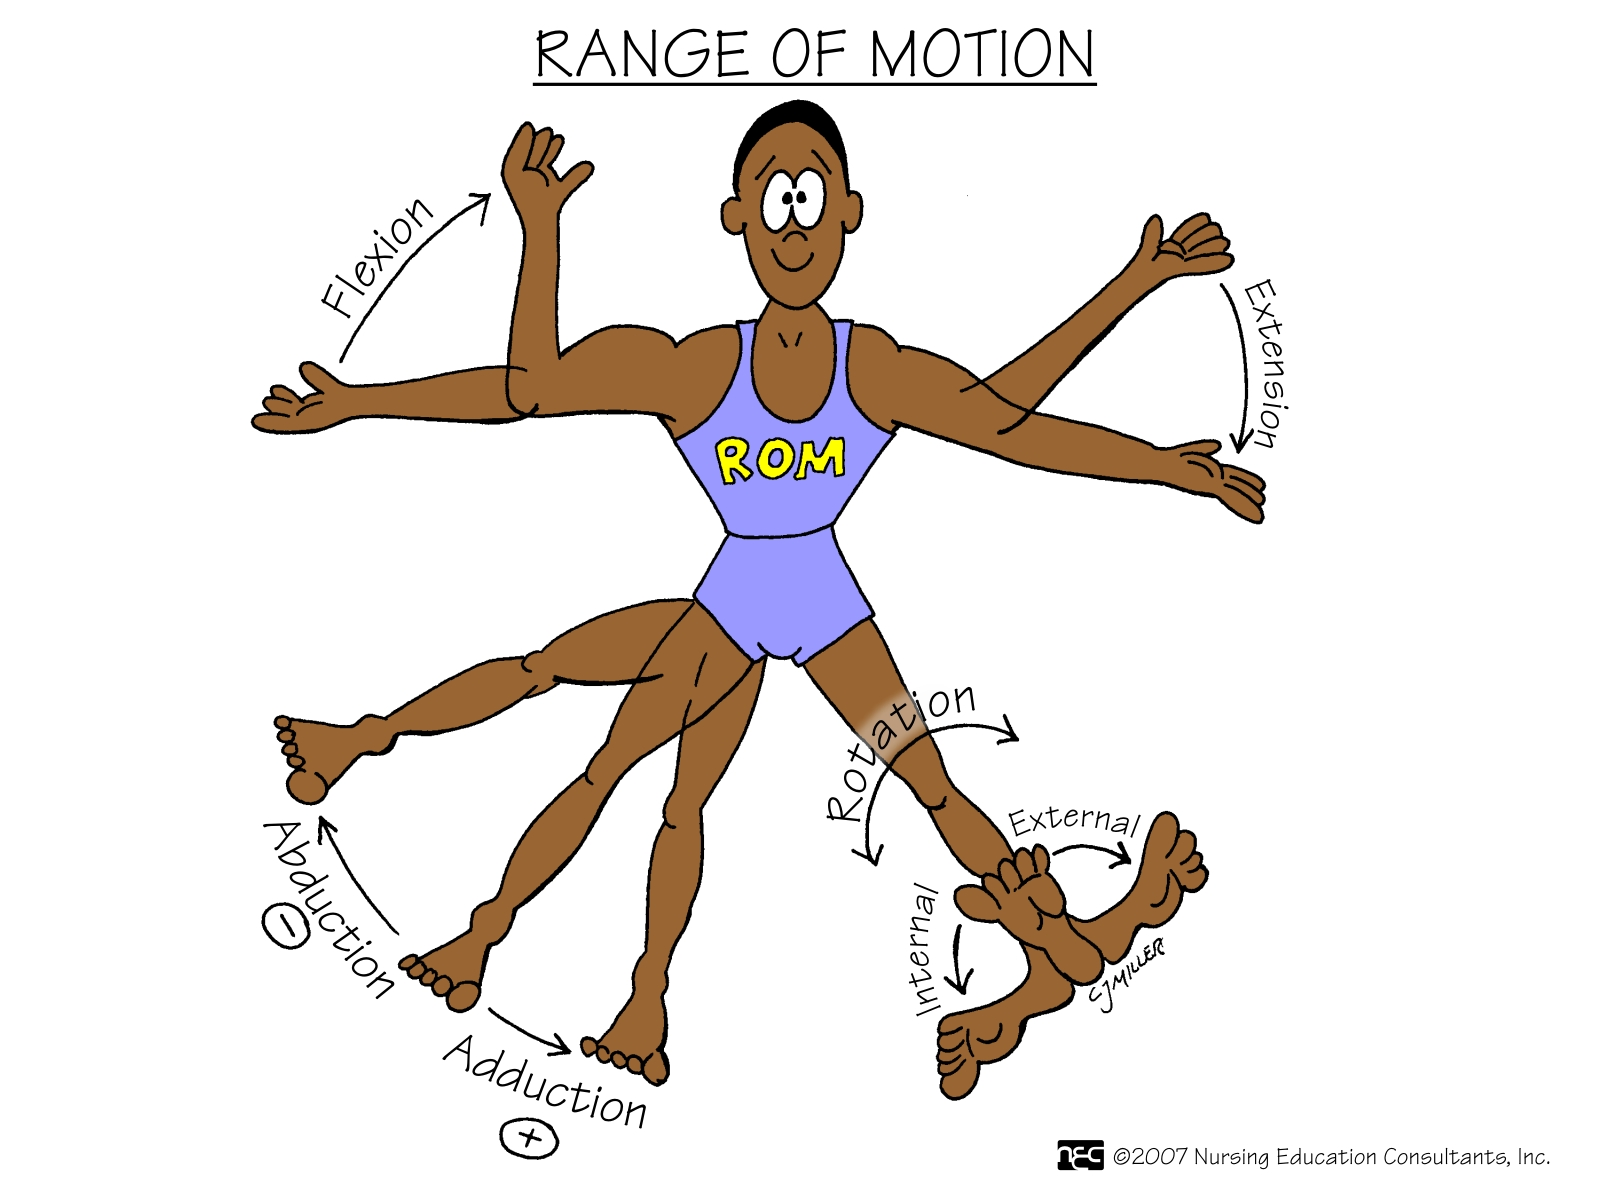
\includegraphics[scale=0.25]{fig/rangeofmotion.png}}  
	\caption{Range of Motion}
\end{figure}

\par The problem is that up to 70\% of patients give up physiotherapy because they can not see immediate results \cite{7FactsInPhysicalTherapy}.
\par That's why we want to make a application which makes use of a camera to objectively calculate ROM in real-time and automatically produce a report that tracks progress over the course of several therapy sessions.

% \section{The purpose of the application}